\documentclass[fleqn]{article}

\usepackage{graphicx}
\usepackage{xurl}
\usepackage{url}
\usepackage{caption}
\usepackage{fancyhdr}
\usepackage{mathtools}
\usepackage{amsmath}
\usepackage{amssymb}
\usepackage{tikz}
\usepackage{listings}
\usepackage{xcolor}
\usepackage{float}

\definecolor{codegreen}{rgb}{0,0.6,0}
\definecolor{codegray}{rgb}{0.5,0.5,0.5}
\definecolor{codepurple}{rgb}{0.58,0,0.82}
\definecolor{backcolour}{rgb}{0.95,0.95,0.92}

\lstdefinestyle{mystyle}{
	backgroundcolor=\color{backcolour},   
	commentstyle=\color{codegreen},
	keywordstyle=\color{magenta},
	numberstyle=\tiny\color{codegray},
	stringstyle=\color{codepurple},
	basicstyle=\ttfamily\footnotesize,
	breakatwhitespace=false,         
	breaklines=true,                 
	captionpos=b,                    
	keepspaces=true,                 
	numbers=left,                    
	numbersep=5pt,                  
	showspaces=false,                
	showstringspaces=false,
	showtabs=false,                  
	tabsize=2
}

\lstset{style=mystyle}

\usepackage{xepersian}

\settextfont[BoldFont={XB Zar bold.ttf}]{XB Zar.ttf}
\setlength\parindent{0pt}

\title{

\includegraphics[width=0.4\textwidth]{sharif.png}\\
\normalsize{دانشکده مهندسی کامپیوتر}\\
\vspace{1cm}
	
\huge{آزمایشگاه طراحی سیستم‌های دیجیتال}
\\
\Large{گزارش آزمایش پنچم}
\\
}

\author{
\\
دکتر سیاوش بیات سرمدی
\\
\\
پارسا محمدیان --- 98102284
}

\date{\today}

\begin{document}

\clearpage\maketitle
\thispagestyle{empty}

\newpage

\pagestyle{fancy}
\lhead{آزمایشگاه طراحی سیستم‌های دیجیتال}

\rhead{پارسا محمدیان}


\tableofcontents

\setcounter{page}{1}

\newpage

\section{مقدمه}

\subsection*{عنوان گزارش}
طراحی ضرب کننده
\subsection*{موضوع}
استفاده از نرم‌افزارهای طراحی به کمک کامپیوتر \footnote{\lr{CAD}} برای طراحی 
و پیاده‌سازی مدار ضرب کننده با الگوریتم بوث.
\subsection*{شرح ابزارها و برنامه‌های مورد استفاده}
در این آزمایش از نرم‌افزار \lr{ISE Desgin Suite} که محصول شرکت \lr{Xilinx} است 
استفاده کرده‌ام.

\section{چارچوب نظری و شرح آزمایش}
طبق خواسته آزمایش، بخش‌های واحد کنترل و مسیر داده را جدا طراحی می‌کنیم. هر دو 
این دو بخش در فایل 
\lr{multiplier.v}
موجود هستند اما برای جداسازی در بلاک‌های 
\lr{always}
 مجزا قرار گرفته‌اند.

\section{تست مدار}
برای تست مدار در ماژول 
\lr{Stimulus.v}
دو عدد را به عنوان ورودی می‌دهیم سپس خروجی را چاپ کرده و بررسی می‌کنیم. 
همانطور که در شکل 
\ref{test}
مشخص است، حاصل ضرب‌های زیر به درستی محاسبه شده است.
\begin{align*}
	2 \times 4 = 8 \\
	7 \times 7 = 49 \\
	6 \times 5 = 30
\end{align*}


\begin{figure}
	\center
	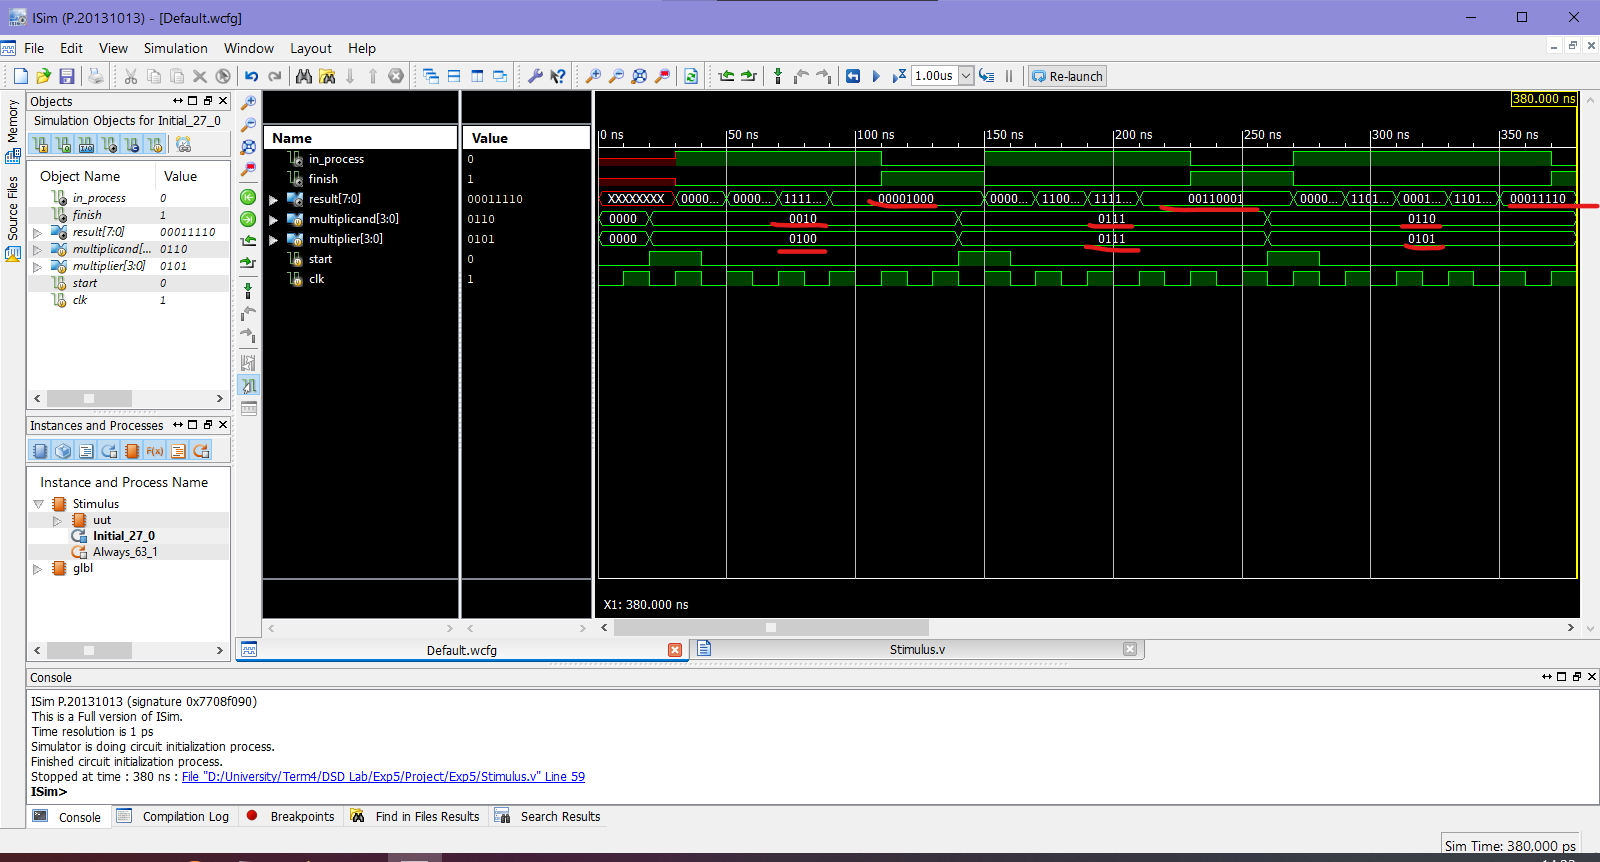
\includegraphics[width=\linewidth]{test.png}
	\caption{تست بنچ مدار}
	\label{test}
\end{figure}


\end{document}
